\section{Experimental Results}
\begin{figure*}[t]
\centering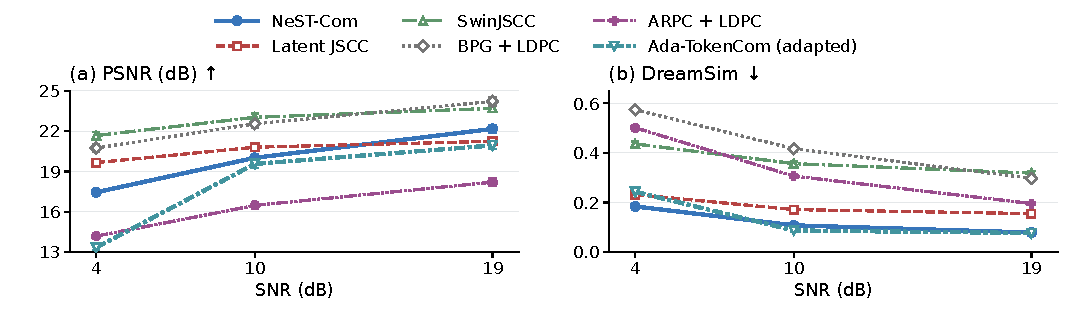
\includegraphics[width=\textwidth]{figure2.pdf}
\caption{Six-system performance on common500 at $N=1024$. Points and error bars are equal-source means and pointwise 95\% source-bootstrap confidence intervals after averaging three channel realizations per source. Ada denotes the predicted-class, fixed-frame adaptation. Higher PSNR and lower DreamSim are favorable.}
\label{fig:performance}
\end{figure*}
\subsection{Experimental Setup}
We use common500 ImageNet validation images~\cite{imagenet}, a disjoint cal1000 set, and Kodak24~\cite{kodak}, with fixed $256\times256$ preprocessing. ImageNet-calibrated policies remain fixed on Kodak. The six-system main study uses $N=1024$; NeST, WHOLE, and Ada also use $N=512$, each independently calibrated at 4/10/19~dB.

Our convolutional Latent JSCC maps tokenizer latents to symbols and shares $\Dc$, using MSE, LPIPS, and latent-consistency losses. It and SwinJSCC~\cite{swinjscc}, adapted to $256\times256$ and $N=1024$, use the same 20\,000 training images and final 100k/200k-update checkpoints. SwinJSCC was still improving at its training cap. Digital baselines are adaptive BPG~\cite{bpg} + LDPC, ARPC~\cite{arpc} + LDPC with paid captions, and predicted-class, fixed-frame Ada~\cite{adatokencom}. Ada retains LlamaGen-L/VQ16 and prefix arithmetic coding. A fixed ConvNeXt predicts the paid 10-bit class ($b+39\leq k_a$); fitting searches all 1--256-token endpoints. Its tail uses CFG=4, $T=1$, top-$k=2000$, top-$p=1$. This adaptation does not reproduce Ada's average-budget controller or ARQ.

Metrics are PSNR, LPIPS-Alex~\cite{lpips}, DreamSim~\cite{dreamsim}, and CLIP ViT-L/14 image--image cosine (CLIP-I)~\cite{clip}. Frozen FP32 preprocessing uses $224\times224$ bicubic-antialias inputs for DreamSim/CLIP. DINOv2-based calibration is related to feature-based evaluation; controlled interventions provide the mechanism evidence. Three original channel outcomes, including gray failures, are averaged per source before equal-source means and direct source-paired 95\% bootstrap intervals (10\,000 resamples). N512 shares source/repeat-specific AWGN across methods; N1024 retains historical noise identities. E1/E2 use the fixed existing 100-source subset and actual received inputs, without new PHY trials or training. They are diagnostics, not new independent test sets.

\subsection{Effect of Within-Scale Endpoints}
\begin{table}[t]
\caption{Within-scale endpoint and receiver evidence. (A) Main family-specific policies; differences are PARTIAL minus WHOLE. (B) Controlled granularity on 100 sources with fixed model, MCS, maximum endpoint and fitting rule. (C) Receiver interventions on the same 100 sources and actual prefixes. Brackets give source-paired 95\% CIs; populations and conditions are as stated.}
\label{tab:internal}
\centering\footnotesize
\setlength{\tabcolsep}{2.5pt}
\begin{tabular}{ccc}
\toprule
\multicolumn{3}{l}{(A) Main policies at $N=1024$} \\
SNR & Util. W$\to$P (\%) & $\Delta$PSNR (dB) [95\% CI] \\
\midrule
\multicolumn{3}{l}{common500} \\
4 & 73.81 $\to$ 93.08 & $+0.616\;[0.564,0.673]$ \\
10 & 77.70 $\to$ 95.21 & $+0.701\;[0.637,0.766]$ \\
19 & 85.24 $\to$ 94.73 & $+0.319\;[0.290,0.349]$ \\
\multicolumn{3}{l}{Kodak24} \\
4 & 75.69 $\to$ 93.43 & $+0.396\;[0.236,0.543]$ \\
10 & 78.11 $\to$ 94.99 & $+0.674\;[0.408,0.958]$ \\
19 & 85.69 $\to$ 93.71 & $+0.228\;[0.140,0.324]$ \\
\midrule
\multicolumn{3}{l}{(B) Fixed-granularity diagnostic, 10 dB} \\
Grid (candidates) & Utilization (\%) & PSNR (dB) \\
Whole (7) & 78.15 & 18.952 \\
Half (13) & 89.21 & 19.396 \\
Quarter (25) & 95.38 & 19.612 \\
Eighth (49) & 97.39 & 19.735 \\
\midrule
\multicolumn{3}{l}{(C) Receiver interventions: $\Delta$PSNR (dB) [95\% CI]} \\
SNR & B0$-$A0 & C0$-$B0 \\
10 & $+0.220\;[0.176,0.264]$ & $+0.440\;[0.330,0.558]$ \\
19 & $+0.301\;[0.247,0.358]$ & $+0.000\;[0.000,0.000]$ \\
\bottomrule
\end{tabular}
\end{table}

Table~\ref{tab:internal}(A) compares WHOLE/PARTIAL with shared tokenizer, prior, entropy coder, and $\Dc$. Separate family calibration selects the same MCS at each SNR. Common500 gains are 0.32--0.70~dB PSNR. At 10~dB, source-bit utilization rises from 77.70\% to 95.21\% and DreamSim falls by 0.0240. Kodak gains 0.674~dB and reduces DreamSim by 0.0164; its 19~dB DreamSim interval includes zero.

Block~B fixes the 100 sources, model, MCS, maximum endpoint, and fitting rule. Eighth adds $0.123\,[0.079,0.169]$~dB over Quarter at 10~dB, but its DreamSim/CLIP-I difference intervals cross zero. Mean terminated-length checks increase from 3.55/5.55/9.49 to 17.58 for Whole/Half/Quarter/Eighth. These checks compare terminated streams, not model forwards or elapsed time; Quarter is predefined.

Block~C uses the same actual prefixes. A0 ignores received boundary tokens and follows the prior. B0 adds their correction to the final residual latent while finer-scale conditioning follows A0. C0 updates both latent and conditioning, on the same device and precision. The ordered PSNR differences are 0.220 and 0.440~dB at 10~dB. At 19~dB, the last-scale boundary leaves no C0$-$B0 increment. A0 still uses completion; these diagnostics do not decompose the common500 gain.

E2 separately compares direct coarse decoding, $R0=\Dc(\sum_{s=1}^{m}C_s(q_s))$, with existing VAR-completed WHOLE output R1 from the identical received prefix. Both retain the original ten-scale transforms, full latent grid, and frozen $\Dc$. R1$-$R0 PSNR is $0.026\,[-0.204,0.271]$~dB at N512, 4~dB, and $0.771\,[0.563,0.986]$~dB at 10~dB. DreamSim changes by $-0.4204\,[-0.4488,-0.3925]$ and $-0.4519\,[-0.4790,-0.4248]$, respectively; LPIPS decreases and CLIP-I increases at both points with intervals excluding zero. Thus completion improves feature quality here, while its PSNR benefit depends on the operating point and adapted decoder.

\subsection{Comparison With Existing Methods}
\begin{table}[t]
\caption{Perceptual distance and image-feature similarity on common500 at $N=1024$. Each cell is LPIPS-Alex$\downarrow$ / CLIP-I$\uparrow$. Ada denotes the fixed-frame adaptation. Values are source means.}
\label{tab:external}
\centering\footnotesize
\setlength{\tabcolsep}{3pt}
\begin{tabular}{lccc}
\toprule Method & 4 dB & 10 dB & 19 dB \\
\midrule
NeST-Com & 0.263 / 0.821 & 0.171 / 0.873 & 0.118 / 0.900 \\
Latent JSCC & 0.219 / 0.741 & 0.173 / 0.789 & 0.158 / 0.804 \\
SwinJSCC & 0.530 / 0.627 & 0.469 / 0.669 & 0.440 / 0.697 \\
BPG + LDPC & 0.725 / 0.586 & 0.589 / 0.635 & 0.458 / 0.684 \\
ARPC + LDPC & 0.512 / 0.644 & 0.341 / 0.713 & 0.250 / 0.788 \\
Ada (adapted) & 0.395 / 0.828 & 0.167 / 0.884 & 0.138 / 0.892 \\
\bottomrule
\end{tabular}
\end{table}

Fig.~\ref{fig:performance} and Table~\ref{tab:external} compare complete systems with different tokenizers, priors, decoders, conditioning, and decoding rules. NeST exceeds Ada in PSNR by 4.116/0.455/1.226~dB at 4/10/19~dB. Ada has better LPIPS, DreamSim, and CLIP-I at 10~dB, higher CLIP-I at 4~dB, and slightly lower DreamSim at 19~dB. At 19~dB Ada transmits all 256 tokens: its approximately 58\% source-capacity utilization reflects a complete representation. SwinJSCC and BPG have higher PSNR than NeST throughout; Latent JSCC has higher PSNR at 4/10~dB and lower LPIPS at 4~dB. NeST's PSNR advantage over ARPC is 3.26--3.97~dB.

E1 changes only Ada's unreceived-tail sampling to argmax, rebuilding context from the received prefix and following the greedy path. At N1024, 10~dB, argmax minus sampling gives $-0.156\,[-0.369,0.057]$~dB PSNR and $+0.0036\,[0.0010,0.0060]$ DreamSim. On these same 100 sources, NeST minus argmax yields $+0.568\,[0.246,0.902]$~dB PSNR but $+0.0178\,[0.0129,0.0229]$ DreamSim; Ada retains higher CLIP-I, while the LPIPS difference interval crosses zero. The original sampling baseline remains in the main comparison.

No rejected or failed reconstructions occurred in the 1500 trials per method at each matched SNR on common500 at N1024. Latent JSCC has no discrete CRC rejection. On Kodak, all four paired metrics favor NeST over Ada at 4~dB; only PSNR excludes zero at 10~dB, and PSNR/LPIPS favor NeST at 19~dB while DreamSim/CLIP-I intervals cross zero.

\subsection{Transmission With a Reduced Symbol Budget}
\begin{figure*}[t]
\centering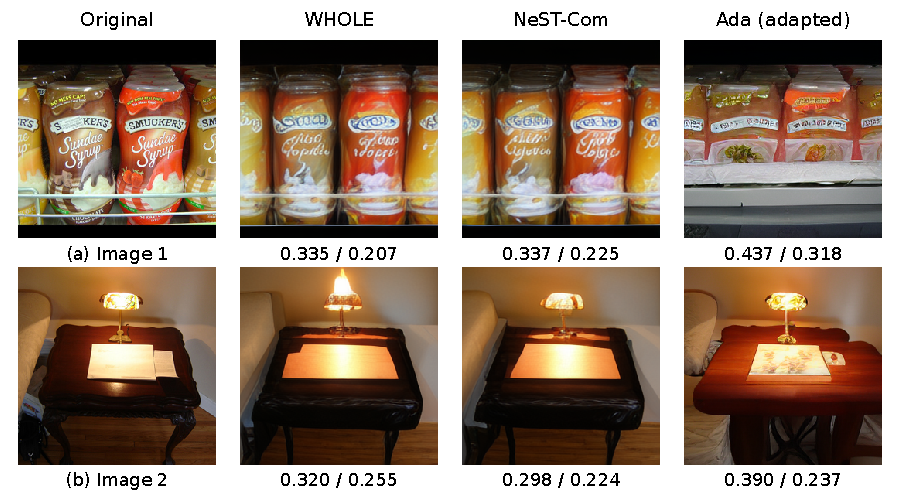
\includegraphics[width=6.0in]{figure3.pdf}
\caption{Source reconstructions at $N=512$ and 10~dB for two images selected by the preregistered source-ID rule. Columns show the original, WHOLE, NeST-Com, and the fixed-frame Ada-TokenCom adaptation. Each reconstruction uses the first registered channel repetition. Values are LPIPS-Alex$\downarrow$ / DreamSim$\downarrow$ for the displayed realization.}
\label{fig:qualitative}
\end{figure*}
\begin{table}[t]
\caption{Reduced-budget comparison on common500 at $N=512$. Differences are NeST-Com minus the fixed-frame Ada-TokenCom adaptation; brackets give source-paired 95\% CIs. Positive PSNR and negative DreamSim favor NeST-Com.}
\label{tab:reduced}
\centering\footnotesize
\setlength{\tabcolsep}{4pt}
\begin{tabular}{ccc}
\toprule SNR & $\Delta$PSNR (dB) & $\Delta$DreamSim \\
\midrule
4 & $+4.180$ & $-0.1029$ \\
 & $[3.991,4.377]$ & $[-0.1142,-0.0917]$ \\
10 & $+4.055$ & $-0.0660$ \\
 & $[3.880,4.235]$ & $[-0.0747,-0.0573]$ \\
19 & $+1.740$ & $+0.0139$ \\
 & $[1.577,1.909]$ & $[0.0103,0.0173]$ \\
\bottomrule
\end{tabular}
\end{table}

At $N=512$, 68 header symbols leave 444 body symbols. WHOLE minus Ada has descriptive PSNR mean differences of 3.79/3.66/0.95~dB at 4/10/19~dB. NeST further improves over WHOLE by $0.392\,[0.341,0.444]$, $0.399\,[0.356,0.445]$, and $0.792\,[0.740,0.844]$~dB; all corresponding LPIPS, DreamSim, and CLIP-I paired intervals also favor NeST. At 10~dB, WHOLE/NeST select the same target $(7,0)$ and 16-QAM rate-2/3 MCS; additional within-scale fallback endpoints raise utilization from 79.30\% to 93.46\%.

NeST has higher PSNR and lower LPIPS than Ada at all three SNRs. DreamSim favors NeST at 4/10~dB and Ada at 19~dB (Table~\ref{tab:reduced}); CLIP-I favors Ada throughout. In Fig.~\ref{fig:qualitative}(a), WHOLE/NeST retain the jar arrangement more closely than Ada, but WHOLE has lower displayed distances than NeST. All methods alter lamp/tabletop details in (b), where NeST has the lowest distances. Individual outcomes differ from the aggregate ranking.

In E1 at N512, argmax reduces Ada PSNR by $0.475\,[0.152,0.801]$ and $0.651\,[0.338,0.984]$~dB at 4/10~dB and worsens all three feature metrics. NeST minus argmax remains $4.632\,[4.183,5.093]$ and $4.600\,[4.188,5.018]$~dB; its LPIPS/DreamSim intervals also favor NeST, while CLIP-I intervals cross zero. This fixed greedy variant preserves the low-budget gap without isolating all model differences.

Main-study body-CRC rejections are 4/7/5 for NeST/WHOLE/Ada at 4~dB, 1/0/0 at 10~dB, and zero at 19~dB, each out of 1500. All remain in the means; no source requires NULL. Independent calibration and different candidate pools preclude attributing cross-budget differences solely to $N$ or representation order.

\subsection{Additional Results and Processing Cost}
At $N=2048$ (100 sources, two paid 1024-symbol subframes), complete representations at 19~dB give NeST $+1.806$~dB PSNR over ARPC, but worse DISTS~\cite{dists}: $+0.0054\,[0.0024,0.0086]$. With WHOLE/PARTIAL policies fixed at 10~dB and true RX noise variance, all 300 receptions per method on 100 sources are rejected at 8~dB; all succeed at 10/12~dB with identical recovered prefixes and images for each source/method.

Mean TX+RX software processing times at 10~dB are 619.71~ms/image for NeST, 42.48 for Latent JSCC, 44.69 for SwinJSCC, 1520.30 for ARPC, and 2293.01 for BPG (RTX PRO~6000, six CPU cores, batch one, 16 development images, three repeats after warm-up). Ada has not been timed under this protocol.
